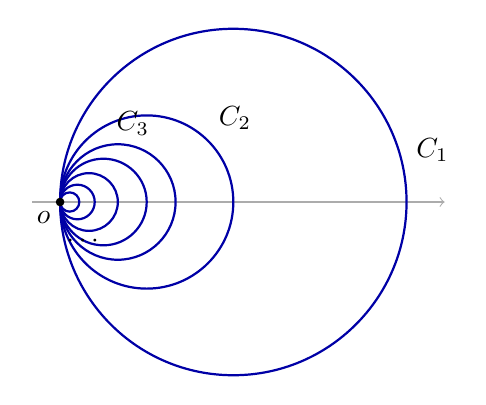
\begin{tikzpicture}[x=2.2cm,y=2.2cm]
	\draw[->,gray!65] (-0.16,0)--(2.22,0);
	\foreach \n in {1,2,3,4,6,10,18}{
		\pgfmathsetmacro{\rad}{1/\n}
		\draw[blue!65!black,thick] (\rad,0) circle[radius=\rad];
	}
	\fill (0,0) circle[radius=0.025];
	\node[below left] at (0,0) {\(o\)};
	\node[right] at (2,0.30) {\(C_1\)};
	\node[above right] at (0.86,0.36) {\(C_2\)};
	\node[above] at (0.42,0.33) {\(C_3\)};
	\node at (0.13,-0.23) {\(\cdots\)};
\end{tikzpicture}
% !TeX root = ../Book1.tex
